\begin{tikzpicture}[line cap=round,line join=round,>=stealth,scale=1.0]
  % Parameters
  \pgfmathsetmacro{\r}{1.6}         % r
  \pgfmathsetmacro{\rho}{4.2}       % rho
  \pgfmathsetmacro{\L}{\rho+0.5*\r} % rho + r/2
  \pgfmathsetmacro{\M}{\rho+1.0*\r} % rho + r
  \pgfmathsetmacro{\R}{\rho+1.5*\r} % rho + 3r/2
  \pgfmathsetmacro{\Xmax}{\rho+3.2*\r}
  \pgfmathsetmacro{\Ymax}{1.15}

  % Axes
  \draw[very thick] (0,0) -- (\Xmax,0) node[below right=2pt] {$|v|$};
  \draw[very thick] (0,0) -- (0,\Ymax);
  % y-axis ticks and labels
  \draw (0,1) -- ++(-0.08,0) node[left] {$1$};
  \node[left] at (0,0) {$0$};

  % Vertical reference lines (dashed)
  \foreach \x/\lab in {%
    \r/{$r$},
    \rho/{$\rho$},
    \L/{$\rho+\tfrac{r}{2}$},
    \M/{$\rho+r$},
    \R/{$\rho+\tfrac{3r}{2}$}}
  {%
    \draw[dashed,black!45] (\x,0) -- (\x,1.02);
    \draw[thick] (\x,0) -- ++(0,-0.06); % small tick on x-axis
    \node[below=6pt] at (\x,0) {\lab};
  }

  % ----- Functions -----
  % eta (magenta): 1 on [0,r], linear to 0 on [r,rho], then 0
  \draw[magenta,very thick] (0,1) -- (\r,1) -- (\rho,0);
  \draw[magenta,very thick] (\rho,0) -- (\Xmax,0); % zero continuation

  % tilde eta (violet): 1 on (-inf, L], linear to 0 on [L,R], then 0
  \draw[violet,very thick] (0,1) -- (\L,1) -- (\R,0) -- (\Xmax,0);

  % 1 - tilde eta (teal): 0 on (-inf, L], linear to 1 on [L,R], then 1
  \draw[teal!60!black,very thick]
    (0,0) -- (\L,0) -- (\R,1) -- (\Xmax,1);

  % Labels for functions
  \node[magenta] at (0.55*\r,1.06) {$\eta$};
  \node[violet]  at (\rho+0.72*\r,0.98) {$\tilde \eta$};
  \node[teal!60!black] at (\rho+2.25*\r,0.98) {$1-\tilde \eta$};

\end{tikzpicture}